\documentclass{article}
\usepackage[utf8]{inputenc}

\title{Chem-131C-Lec18}

\author{swflynn}
\date{May 2017}

\usepackage{natbib}
\usepackage{graphicx}
\usepackage{braket}
\usepackage{amsmath}
\usepackage[margin=0.7in]{geometry}
\usepackage{subfigure}
\usepackage{url}
\usepackage{float}

\begin{document}

\maketitle

\section*{Lecture 18; 5/17/17}
We are now going to begin discussing Phase Transitions.
Consider the trajectory a system as we add energy (as heat).
\begin{figure}[H]
    \centering
    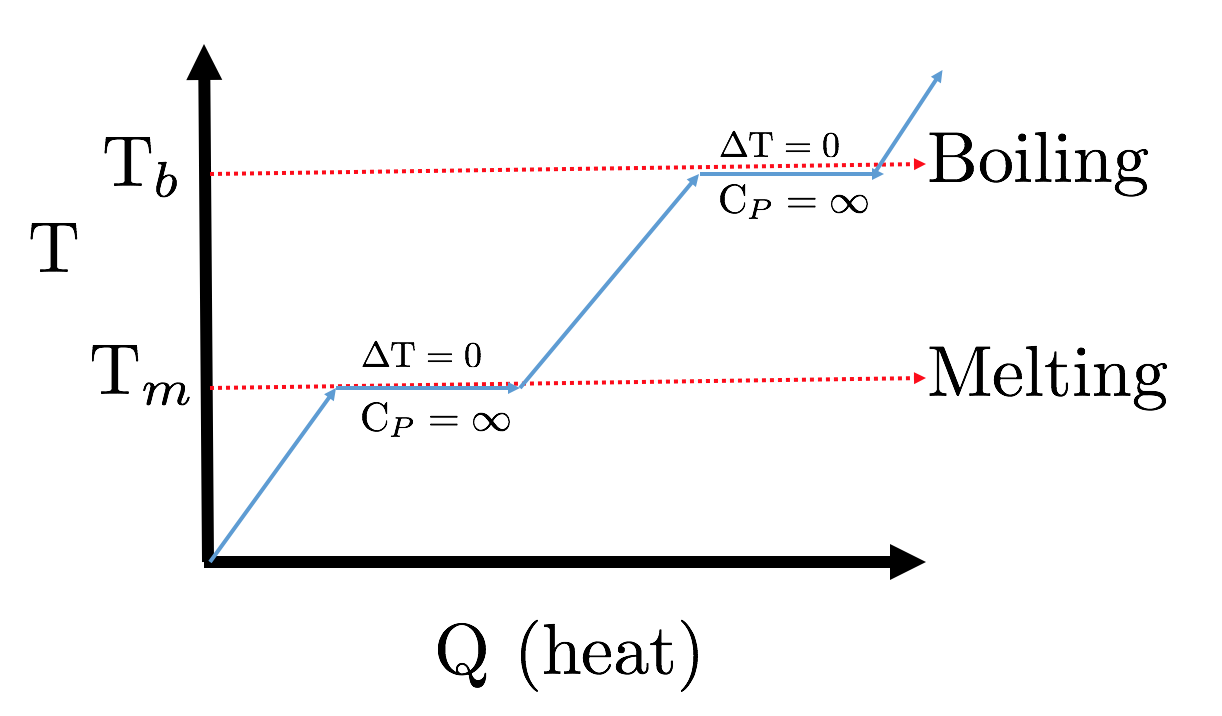
\includegraphics[width=12cm]{phases.png}
    \caption{'Heating Trajectory'. The energy entering the system raises the temperature of the atoms until we reach a phase transition. At the phase transition all of the energy is used for the physical transition process, and there is no temperature change. This is characterized by an infinite heat capacity. }
    \label{fig:phases}
\end{figure}

\subsection*{Gibbs Potential}
We know that Temperature and Pressure are the characteristic variables for the Gibbs Free Energy.
If we are interested in learning about our system, it is natural to plot G(P) and G(T). 
If we consider a constant pressure process we can write the following
\begin{equation}
    dG = -SdT + VdP = -SdT
\end{equation}
Subsequently we should expect a linear dependence between the Gibbs Free Energy and Temperature with a negative slope of S; See Figure \ref{fig:gibbs}. 
\begin{figure}[! h]
    \centering
    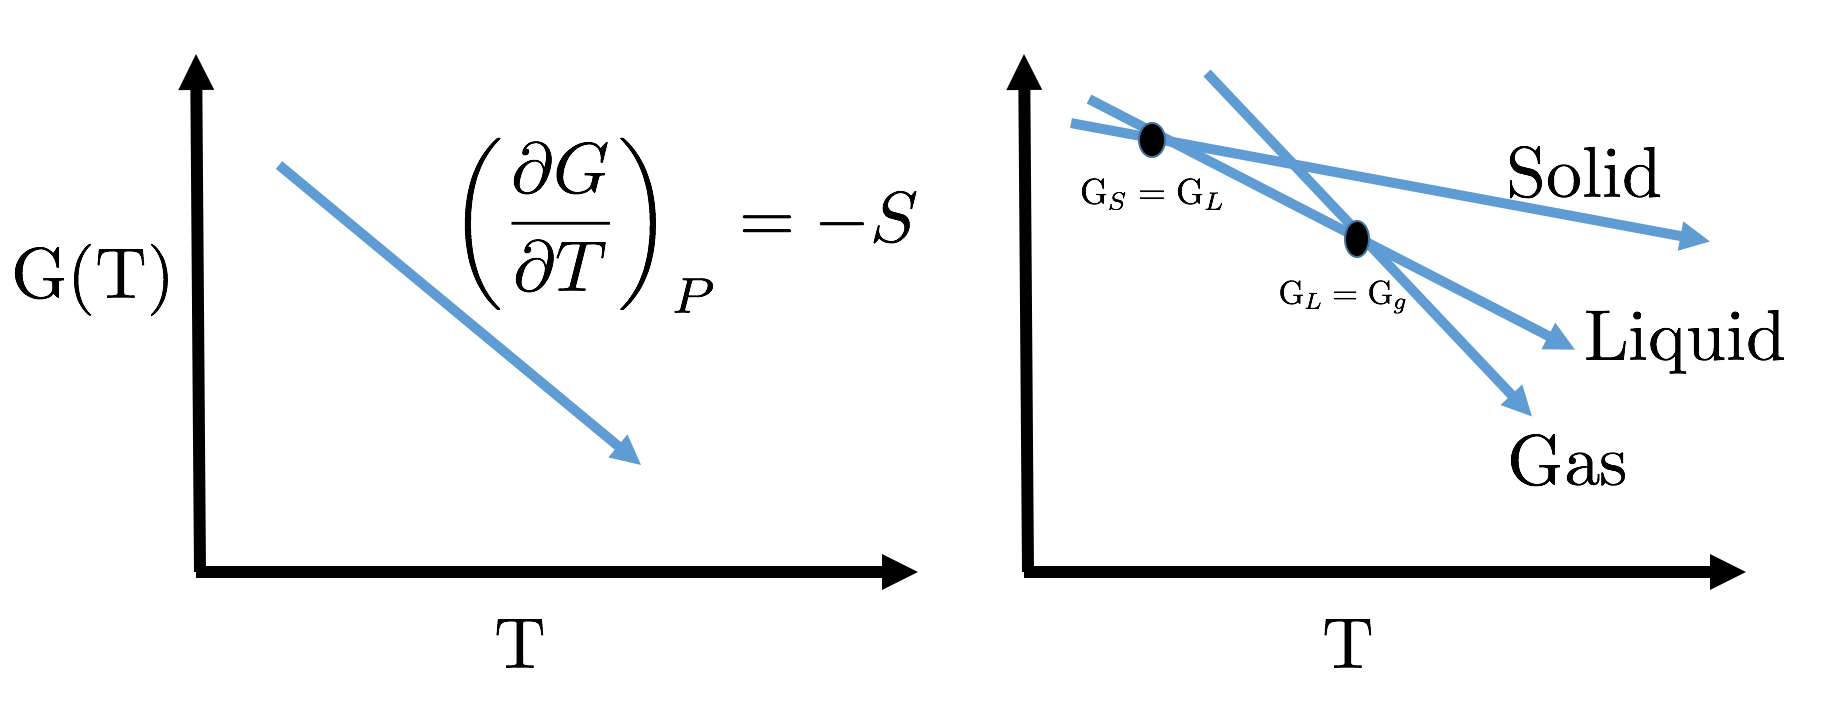
\includegraphics[width=15cm]{gibbs.png}
    \caption{'G(T)$\mid_P$'. We expect the entropy to be greater than 0 for a spontaneous process, with increasing temperature. Therefore the Gibbs Free Energy is less than 0 for a spontaneous process while increasing temperature, holding Pressure constant.}
    \label{fig:gibbs}
\end{figure}

When we consider the change in energy wrt temperature we are discussing the heat capacity. 
The heat capacity of different materials will have different values (and real materials have temperature dependent heat capacities). 
If we plot these different phases on a G(T) vs T plot like above we can guess that a solid will have a shallow dependence, and a gas will have a steep dependence intuitively (again the slope of the line is the entropy). 
The entropy of the same amount of material in the gas state should be higher than a solid because the number of accessible micro-states increases. 
So the slope of each line changes based on the phase, because each phase has an intuitively different entropy. 

By definition, if we have phase coexistence (sitting on the line) than the two phases must have equivalent Gibbs Free Energies.
\begin{equation}
    G_\alpha = G_\beta
\end{equation}
The state with the lowest Gibbs Free Energy is favored. 

\subsection*{Freezing and Melting}
During the physical phase transition between solid to liquid, or liquid to gas, we do not change the temperature.
This means there is no change in the $\Delta$G(T). 
We also know that on this line the Gibbs Free Energy of the 2 physical states must be equal. 
\begin{equation}
\begin{split}
    \Delta_{fus}G &= 0 = \Delta _{fus}H - T\Delta_{fus}S \\
    T_{fus} &= \frac{\Delta _{fus}H}{\Delta _{fus}S}
    \end{split}
\end{equation}
The analogous statement will also be true at the boiling/vaporization interface
\begin{equation}
T_b = T_{vap} = \frac{\Delta _{vap}H}{\Delta _{vap}S}
\end{equation}

\subsection*{Chemical Potential}
If we want to start studying more interesting systems (such as mixing of different chemical species) we need to start tracking their amounts (number moles, concentration, whatever you want) in our fundamental equations G(T,P,n$_1$, $\cdots$ n$_c$) for a system of c-components. 
We can now construct our fundamental equation by simply adding in another term considering all of the components within the system. 
\begin{equation}
\begin{split}
dG &= -SdT + VdP + \sum_{j=1}^{c} \left(\frac{\partial G}{\partial n_j}\right)_{T,P,n_i}dn_i \\
dG &\equiv -SdT + VdP + \sum_{j=1}^c \mu_jdn_j \\
\mu_i &\equiv \left(\frac{\partial G}{\partial n_j}\right)_{T,P,n_i}
\end{split}
\end{equation}
So all we are doing is defining the chemical potential $\mu$ as a sum over all of the partial derivatives of the thermodynamic potential wrt a single component of the system, holding the remainder of the system constant. 
 Consider the simplest system, a 1-component system.
 We can simply normalize by the amount of that 1 component and write the molar Gibbs Free Energy; $\overline{G}$ (note a line over a quantity will refer to a molar quantity, a quantity divided by n).
 \begin{equation}
 \mu = \left(\frac{\partial G}{\partial n}\right)_{T,P} \equiv \overline{G} = \frac{G}{n}
 \end{equation}

\subsection*{Phase Diagrams}
There are various ways to draw phase diagrams, depending on what type of question you are trying to answer.
Consider a P,T diagram as shown. 
These types of diagrams are characterized by critical points, triple points, and will contain various phases depending on the materials being studied.

\begin{figure}[! h]
    \centering
    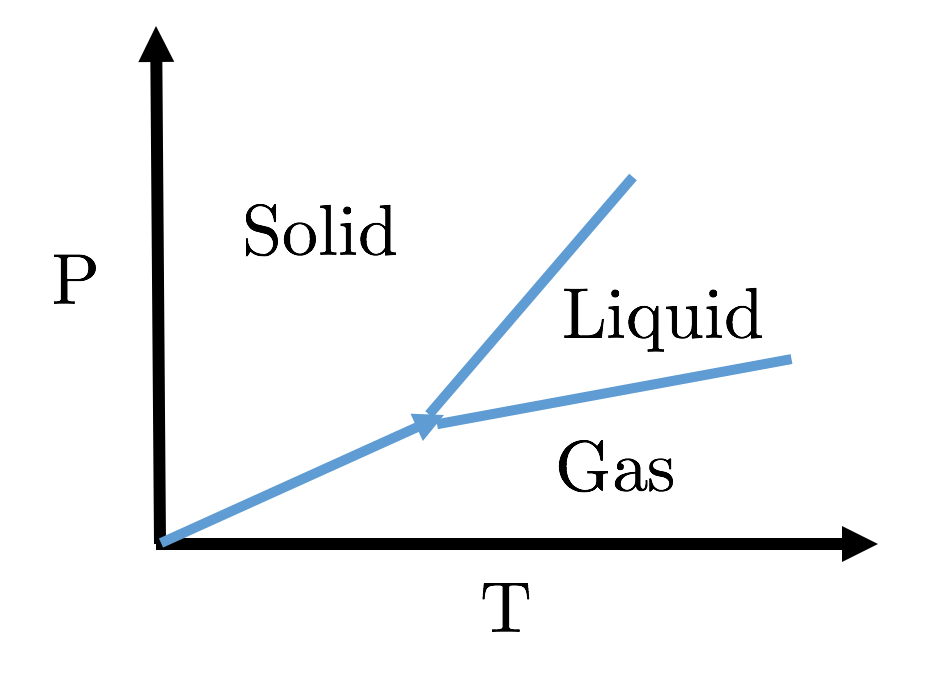
\includegraphics[width=8cm]{p_diag.png}
    \caption{Phase Diagram.The lines on the graph refer to coexistence between the phases. On these coexistence lines we have the chemical potential of the 2 phases being equal, there are in equilibrium.}
    \label{fig:p_diag}
\end{figure}

\subsection*{Chemical Potential}
A potentially new type of graph would be the chemical potential.
If we plot the density dependence of the chemical potential (constant T,P) it begins to look like a reaction coordinate. 

\begin{figure}[! h]
    \centering
    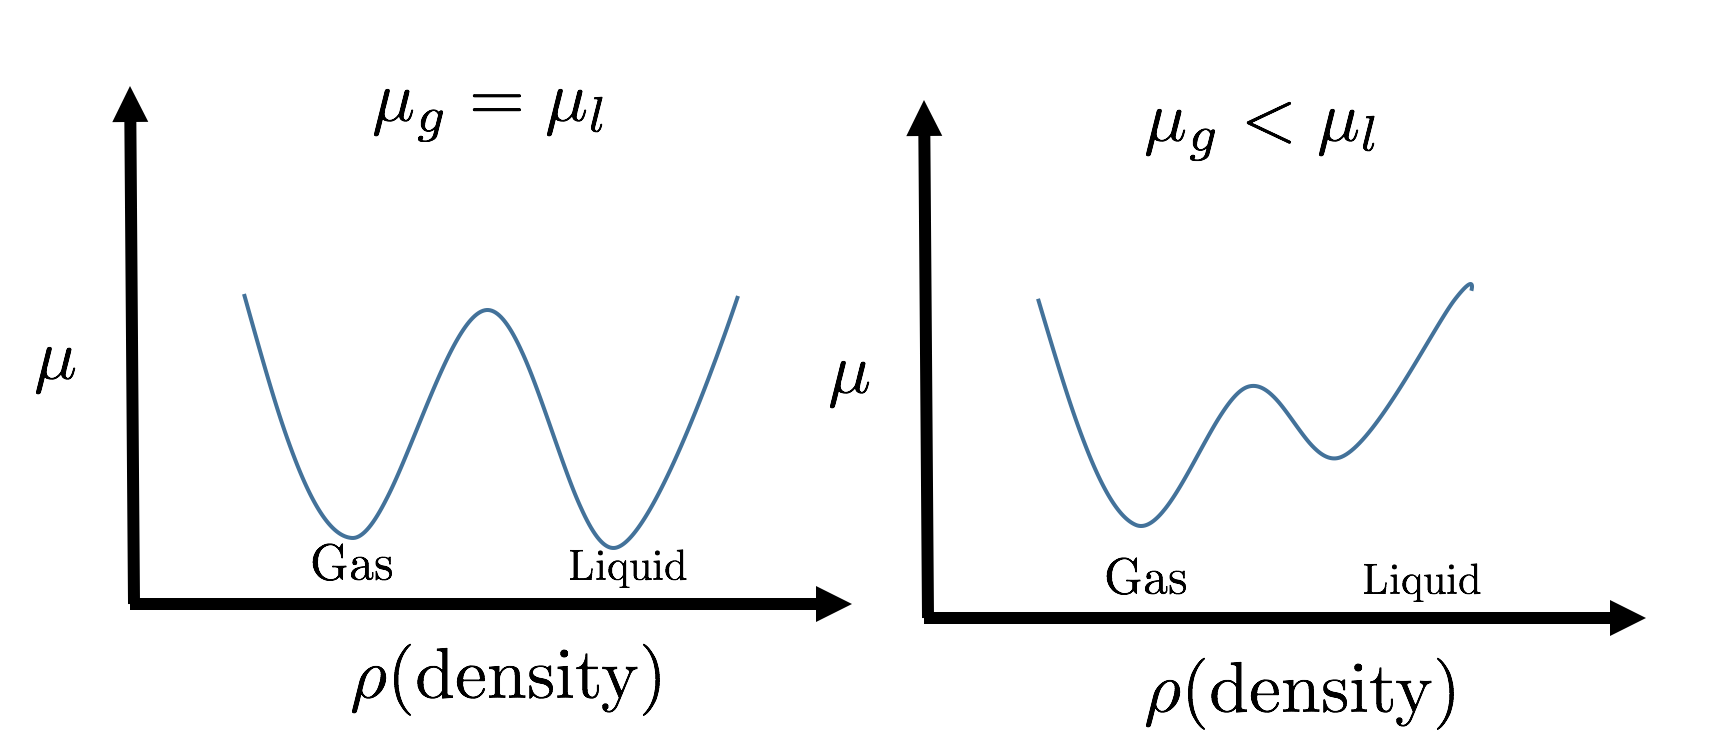
\includegraphics[width=14cm]{chem.png}
    \caption{Reaction Coordinates. As you transition between physical states the chemical potential will decrease for the most favorable state. At equilibrium the chemical potential of the states must be equal.}
    \label{fig:chem}
\end{figure}

There reaction coordinate type plots are a useful way to interpret the super-critical region of a phase diagram.
As we can see there is some barrier that exists between the different physical phases.
When the minimum of a barrier decreases it becomes more likely for the system to be within that state. 
The super-critical region of the phase diagram can be through of as a 'barrier-less' function. 
Without a barrier there is no incentive to be in either state, therefore we get some type of blended super-critical state that will have unique properties when compared to the two standard physical states. 

\begin{figure}[! h]
    \centering
    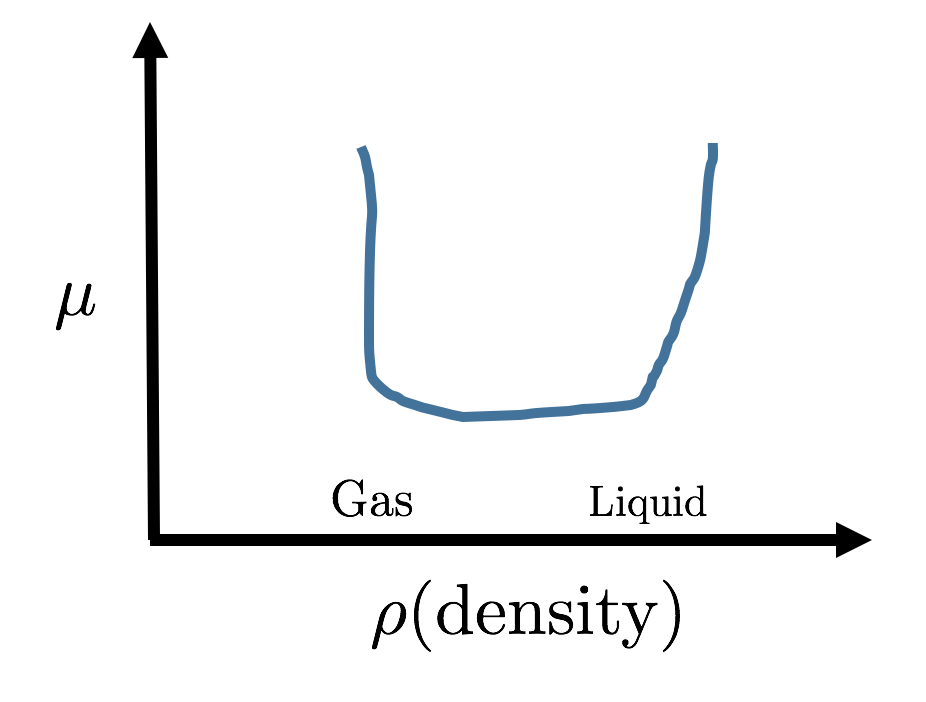
\includegraphics[width=8cm]{super.png}
    \caption{Super-critical Phase. A phase where the barrier between the two physical states no longer exists, you are left with some new type of physical state.}
    \label{fig:super}
\end{figure}

\subsection*{Molar Quantities}
If we consider a phase diagram where we keep constant pressure and study G(T) between T$_A$ and T$_B$ (a phase transition occurs between these temperatures) we can construct various interpretations of molar quantities during the phase transition. 

\begin{figure}[! h]
    \centering
    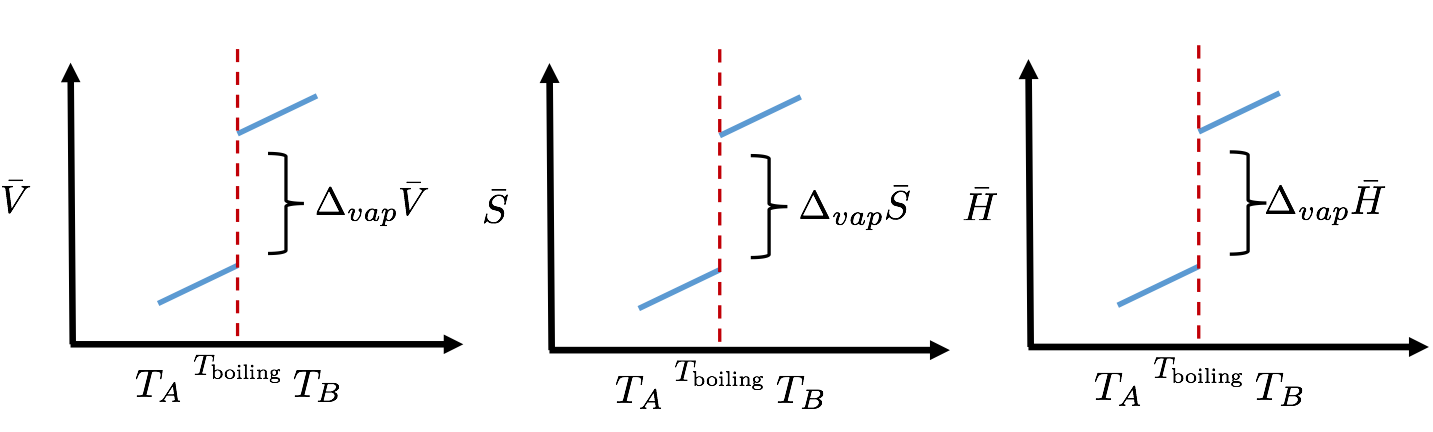
\includegraphics[width=17cm]{molar.png}
    \caption{Molar Quantities. During the phase transition we see discontinuous jumps for various thermodynamic properties.}
    \label{fig:molar}
\end{figure}
We can use these types of graphs to predict the boiling temperature
\begin{equation}
    T_B = \frac{\Delta_{vap}\bar{H}}{\Delta_{vap}\bar{S}}
\end{equation}

If we were to plot the molar Gibbs Free Energy there would not be a discontinuity because the chemical potentials of the two species are actually equal during the transition. 

\end{document}